\documentclass[12pt]{article}

\usepackage[margin=1in]{geometry}
\usepackage{amsmath}
\usepackage{booktabs}
\usepackage{float}
\usepackage{graphicx}
\usepackage{xcolor}

\graphicspath{{figures/}}

\newcommand{\studentname}{KARTHIKEYAN M}
\newcommand{\registernumber}{26120004}
\newcommand{\teammatename}{MIRTHULA R}
\newcommand{\teammateregister}{261200121}
\newcommand{\submissionmonth}{AUGUST 2026}

% Replace each prompt with your own short observation before submission.
\newcommand{\todo}[1]{%
  \par\noindent
  \textcolor{red}{\textbf{[WRITE HERE:} \textit{#1}\textbf{]}}
  \par
}

\begin{document}

\begin{titlepage}
\centering
\vspace*{2cm}
{\Large \textbf{ASSIGNMENT REPORT-3}}\\[2cm]

\textbf{Submitted by :}\\[0.3cm]
\textbf{\studentname} \ [\registernumber]\\[0.3cm]
\textbf{\teammatename} \ [\teammateregister]\\[2cm]

\textbf{Under the guidance of :}\\[0.3cm]
\textbf{HEMA ARUNACHALAM MURTHY}\\[1.5cm]

\textbf{For The Subject}\\[0.5cm]
{\Large \textbf{Pattern Recognition and Machine Learning}}\\[0.3cm]
\textbf{(26AI5707)}\\[3cm]

\vfill
\textbf{DEPARTMENT OF COMPUTER SCIENCE \& ENGINEERING}\\[0.3cm]
\textbf{SHIV NADAR UNIVERSITY}\\[0.3cm]
\textbf{KALAVAKAM}\\[1.5cm]
\textbf{\submissionmonth}
\end{titlepage}

\section*{INTRODUCTION}

This assignment is mainly about Polynomial Regression. We were given a data with non-linear relationship. The assignment requires us to utilize the help of polynomial basis functions and create a design matrix and transform the inputs and then learn the weights in the transformed space. We will look into that visually later. We have also performed some extra experiments like trying out what happens when you don't normalize your data and also tried a different basis function like Gaussian Basis, that has been asked in the last short exam.

\section*{DATA AND SPLIT}

\begin{table}[H]
  \centering
  \caption{Dataset and split used for model selection.}
  \begin{tabular}{lrr}
    \toprule
    Set & Samples & Percentage \\
    \midrule
    Training & 6000 & 60\% \\
    Validation & 2000 & 20\% \\
    Test & 2000 & 20\% \\
    \bottomrule
  \end{tabular}
\end{table}

\begin{figure}[H]
  \centering
  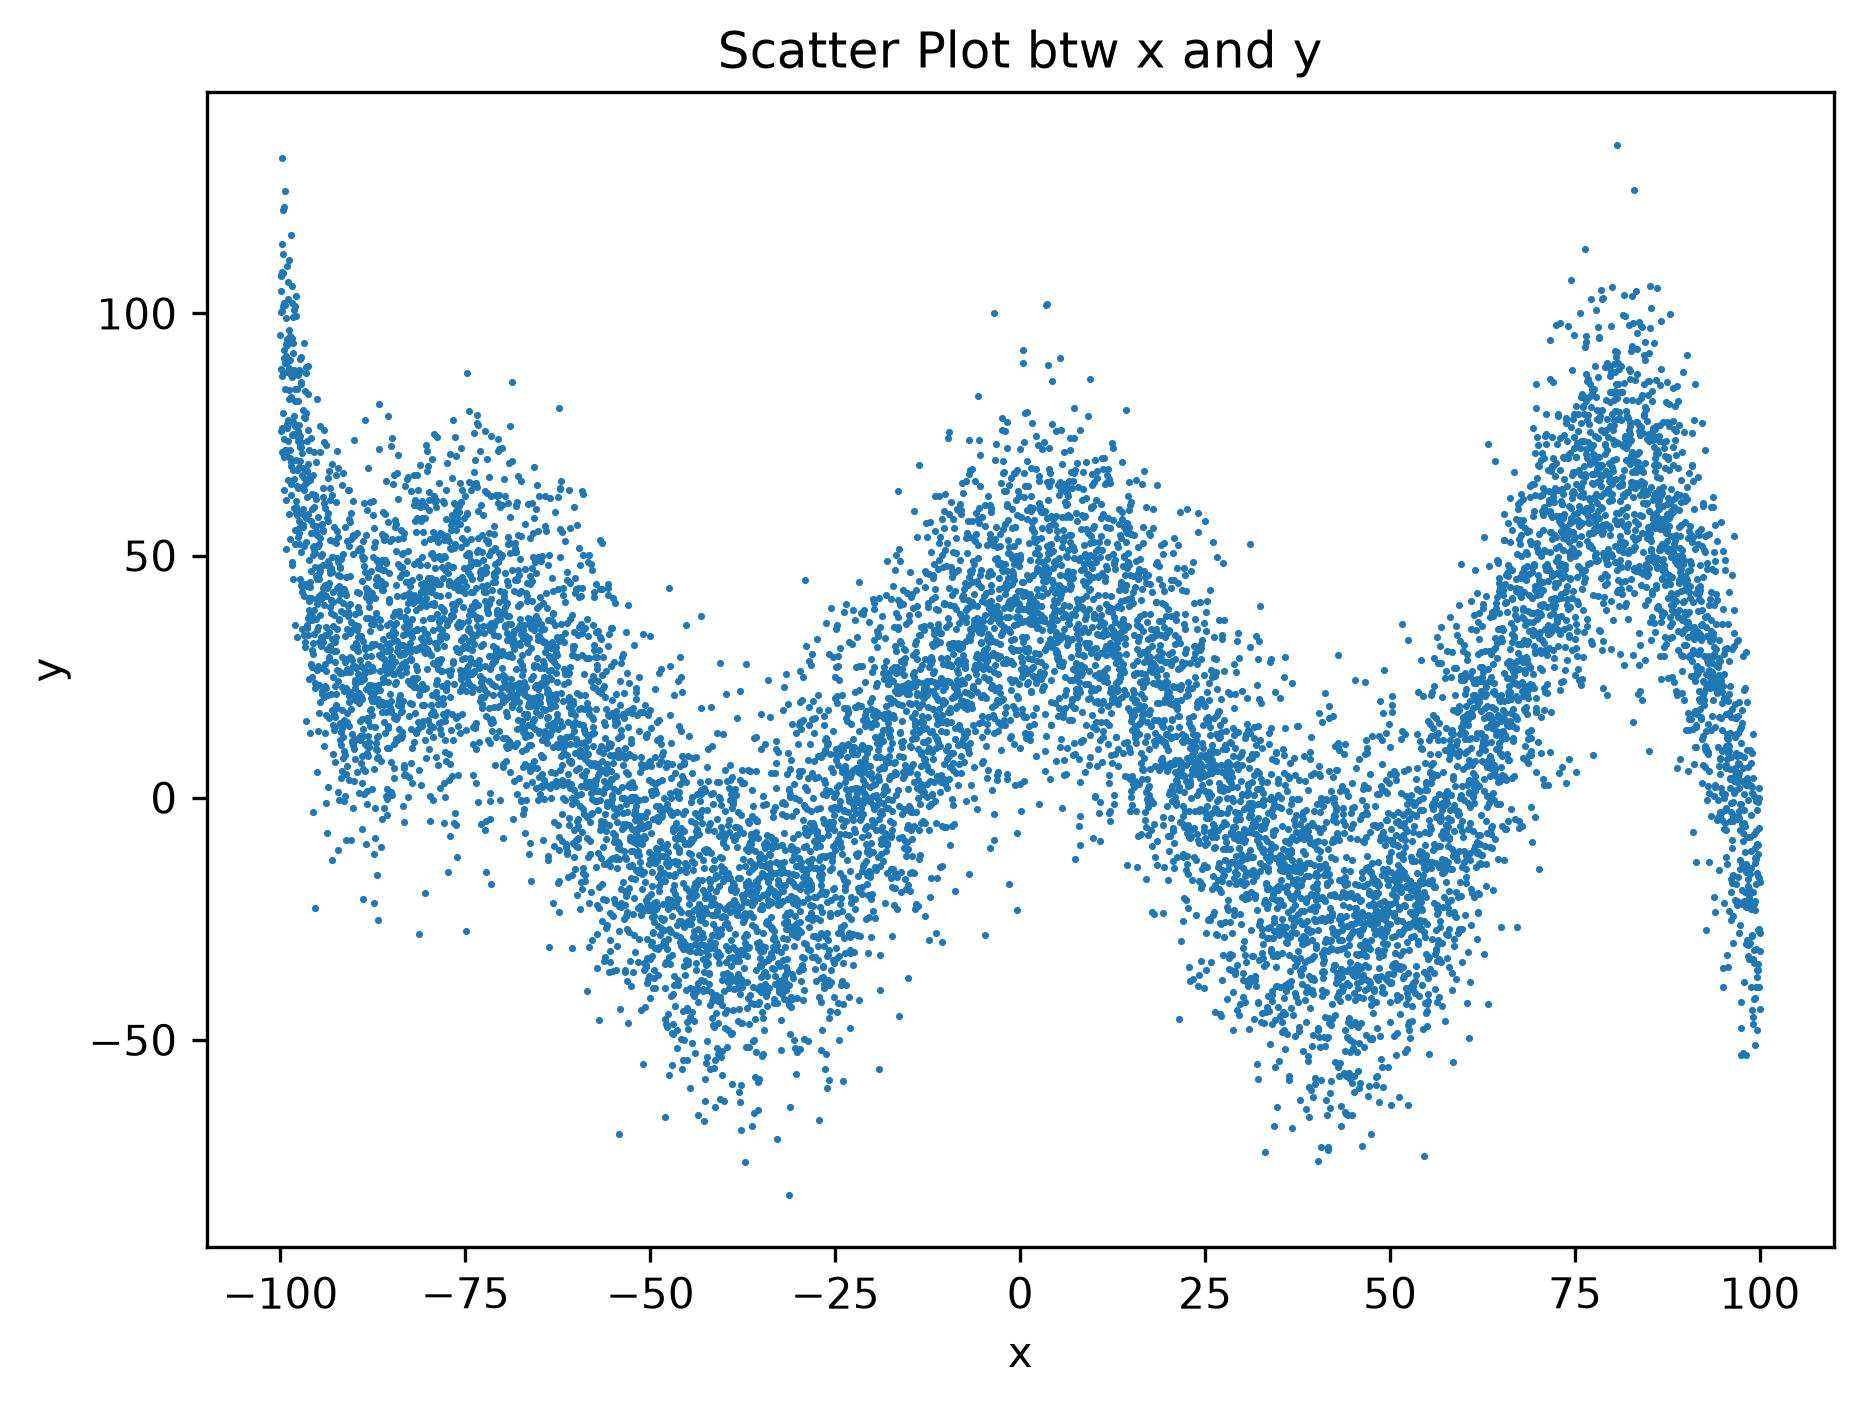
\includegraphics[width=0.80\textwidth]{data_scatter.png}
  \caption{Scatter plot of the 10,000 input--target pairs.}
  \label{fig:data-scatter}
\end{figure}

The given data are clearly non-linear in nature. Thus, a normal linear regression would not be sufficient. Also, when splitting the shuffling part is crucial because without it we would get cut off within a range and will never get the full representation of the data points. Thus, the samples were shuffled with seed 42 before splitting.

\begin{figure}[H]
  \centering
  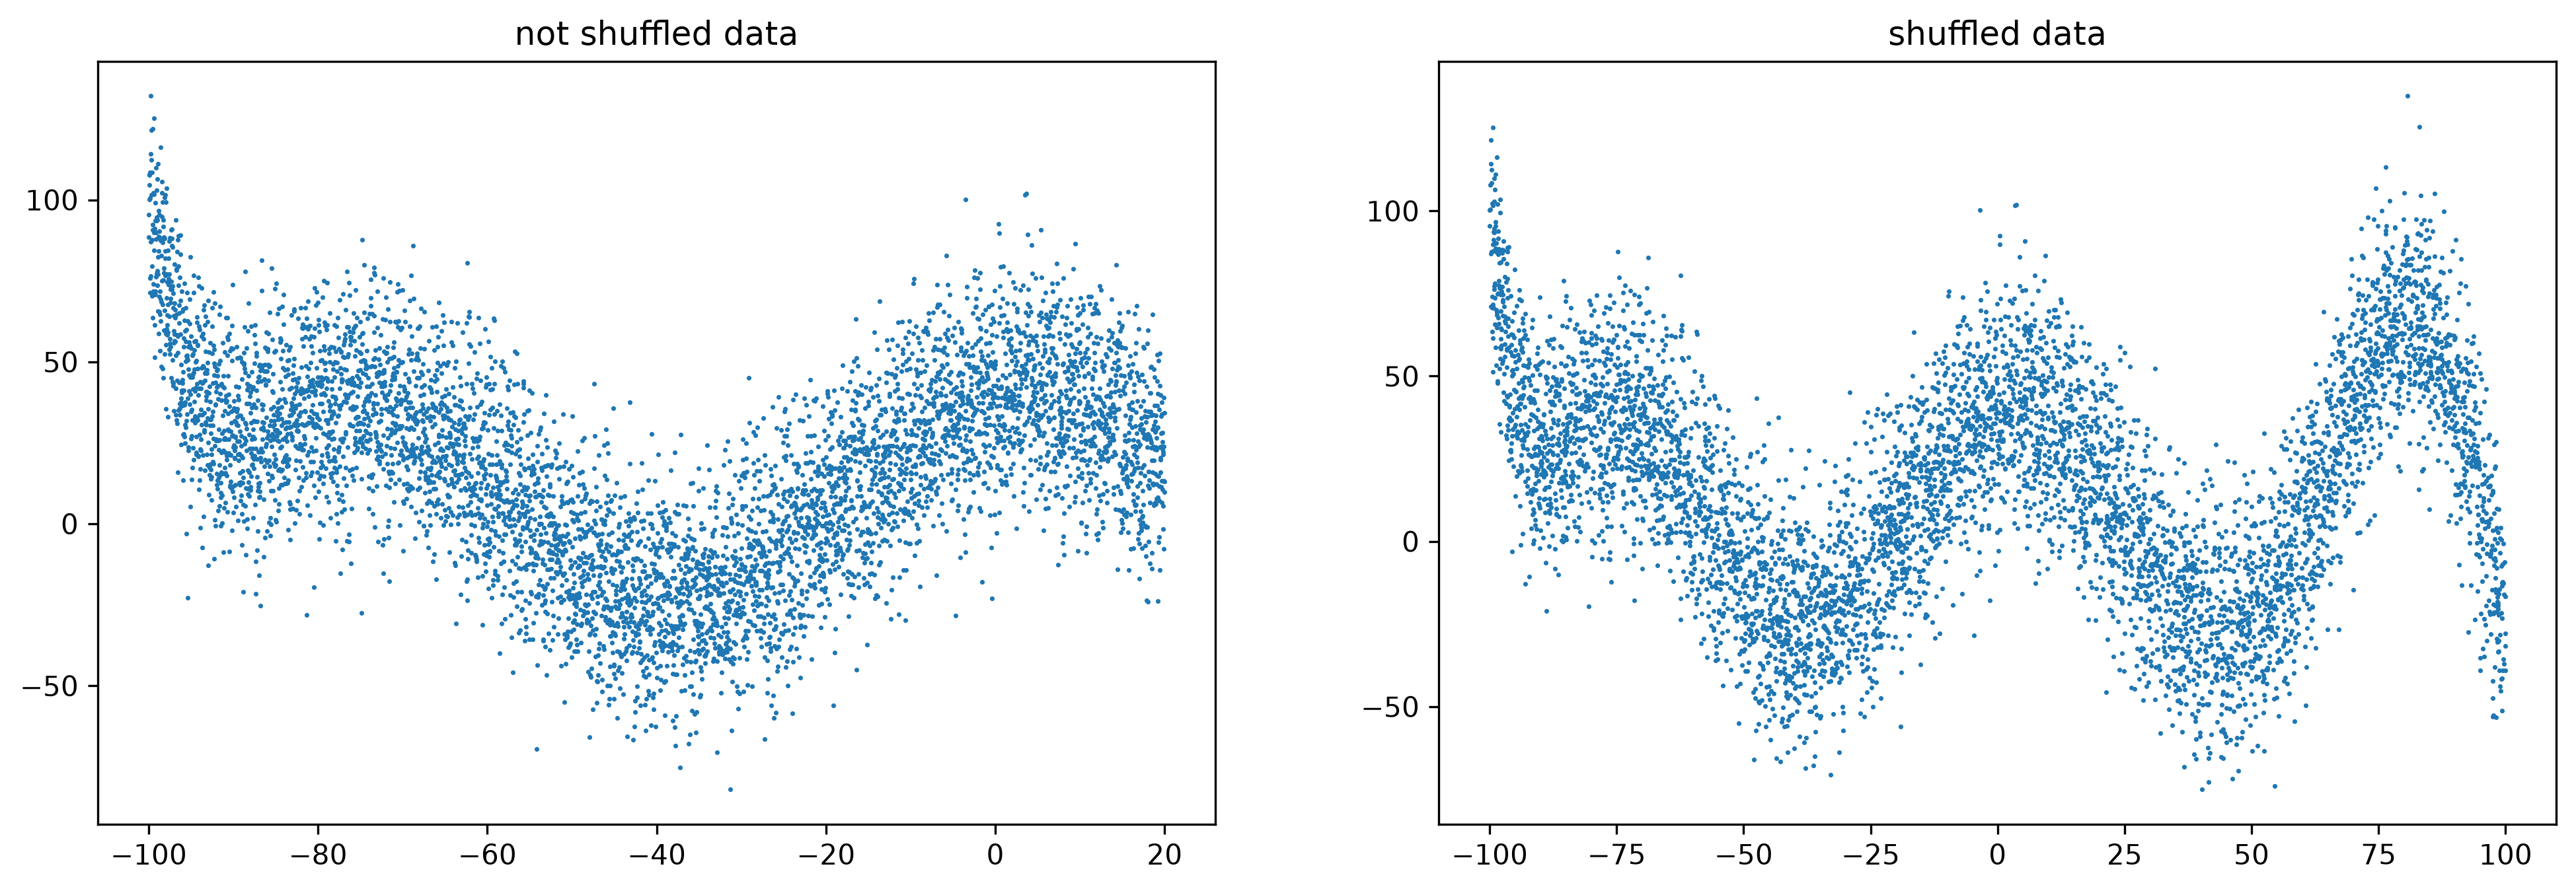
\includegraphics[width=0.94\textwidth]{shuffle_comparison.png}
  \caption{Sample order before and after shuffling.}
  \label{fig:shuffle}
\end{figure}

\section*{POLYNOMIAL REGRESSION}

\subsection*{Basis and least-squares solution}

For degree $d$, the design matrix looks something like this and the each feature is standardized.

\begin{equation}
  \boldsymbol{\phi}(z)=\begin{bmatrix}1&z&z^2&\cdots&z^d\end{bmatrix}^{\mathsf T},
  \qquad z=\frac{x-\mu_x}{\sigma_x}.
  \label{eq:poly-basis}
\end{equation}

The target variable is also scaled to match the input scale $t=(y-\mu_y)/\sigma_y$.

\begin{equation}
  \Phi_{nj}=\phi_j(z_n),
  \qquad \hat{t}(z,\mathbf{w})=\mathbf{w}^{\mathsf T}\boldsymbol{\phi}(z).
  \label{eq:design}
\end{equation}

The weights are obtained by solving for least squares:

\begin{equation}
  \mathbf{w}_{\mathrm{ML}}
  =(\boldsymbol{\Phi}^{\mathsf T}\boldsymbol{\Phi})^{-1}
    \boldsymbol{\Phi}^{\mathsf T}\mathbf{t}.
  \label{eq:least-squares}
\end{equation}

We start with a single input vector {x} and output {y}. We then standardize the data, We transform our inputs using a polynomial basis and then we solve for the least squares solution. We will talk about normalization in more detail in the additional experiments section.
\subsection*{Degree selection}

We experimented different degrees of polynomial (i.e.) from 1 to 15 in order to choose the best degree of polynomial, which is decided via calculating MSE (Mean Squared Error) for each one of those degrees.

\begin{equation}
  \mathrm{MSE}=\frac{1}{N}\sum_{n=1}^{N}(y_n-\hat{y}_n)^2.
\end{equation}

\begin{figure}[H]
  \centering
  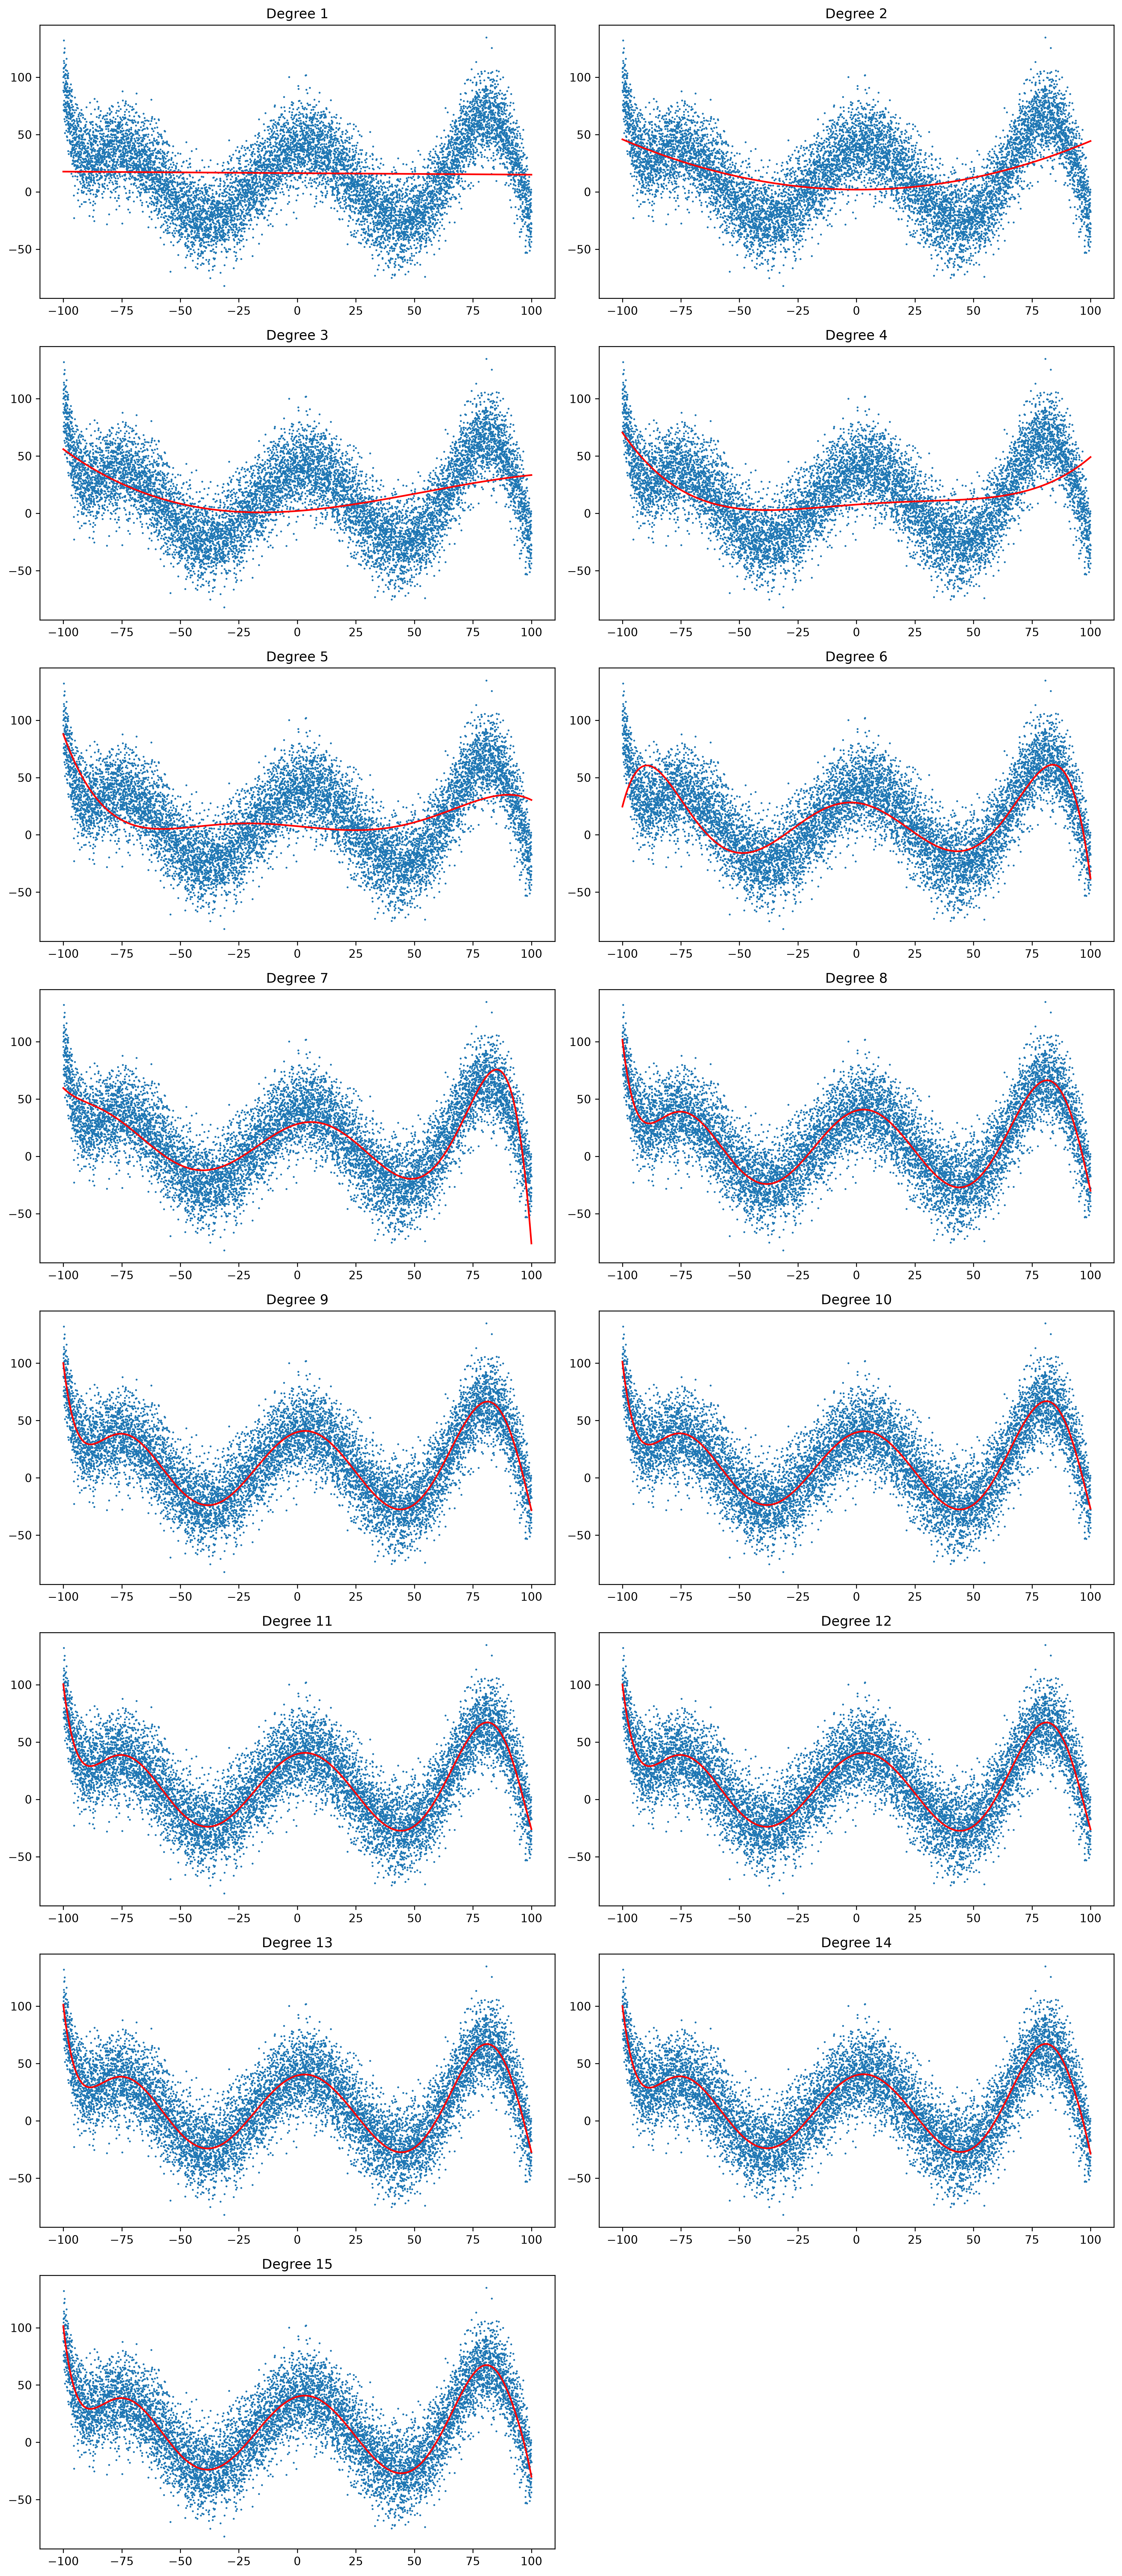
\includegraphics[height=0.9\textheight,keepaspectratio]{polynomial_fits_degrees_1_to_15.png}
  \caption{Polynomial fits for degrees 1 to 15.}
  \label{fig:poly-fits}
\end{figure}

\begin{figure}[H]
  \centering
  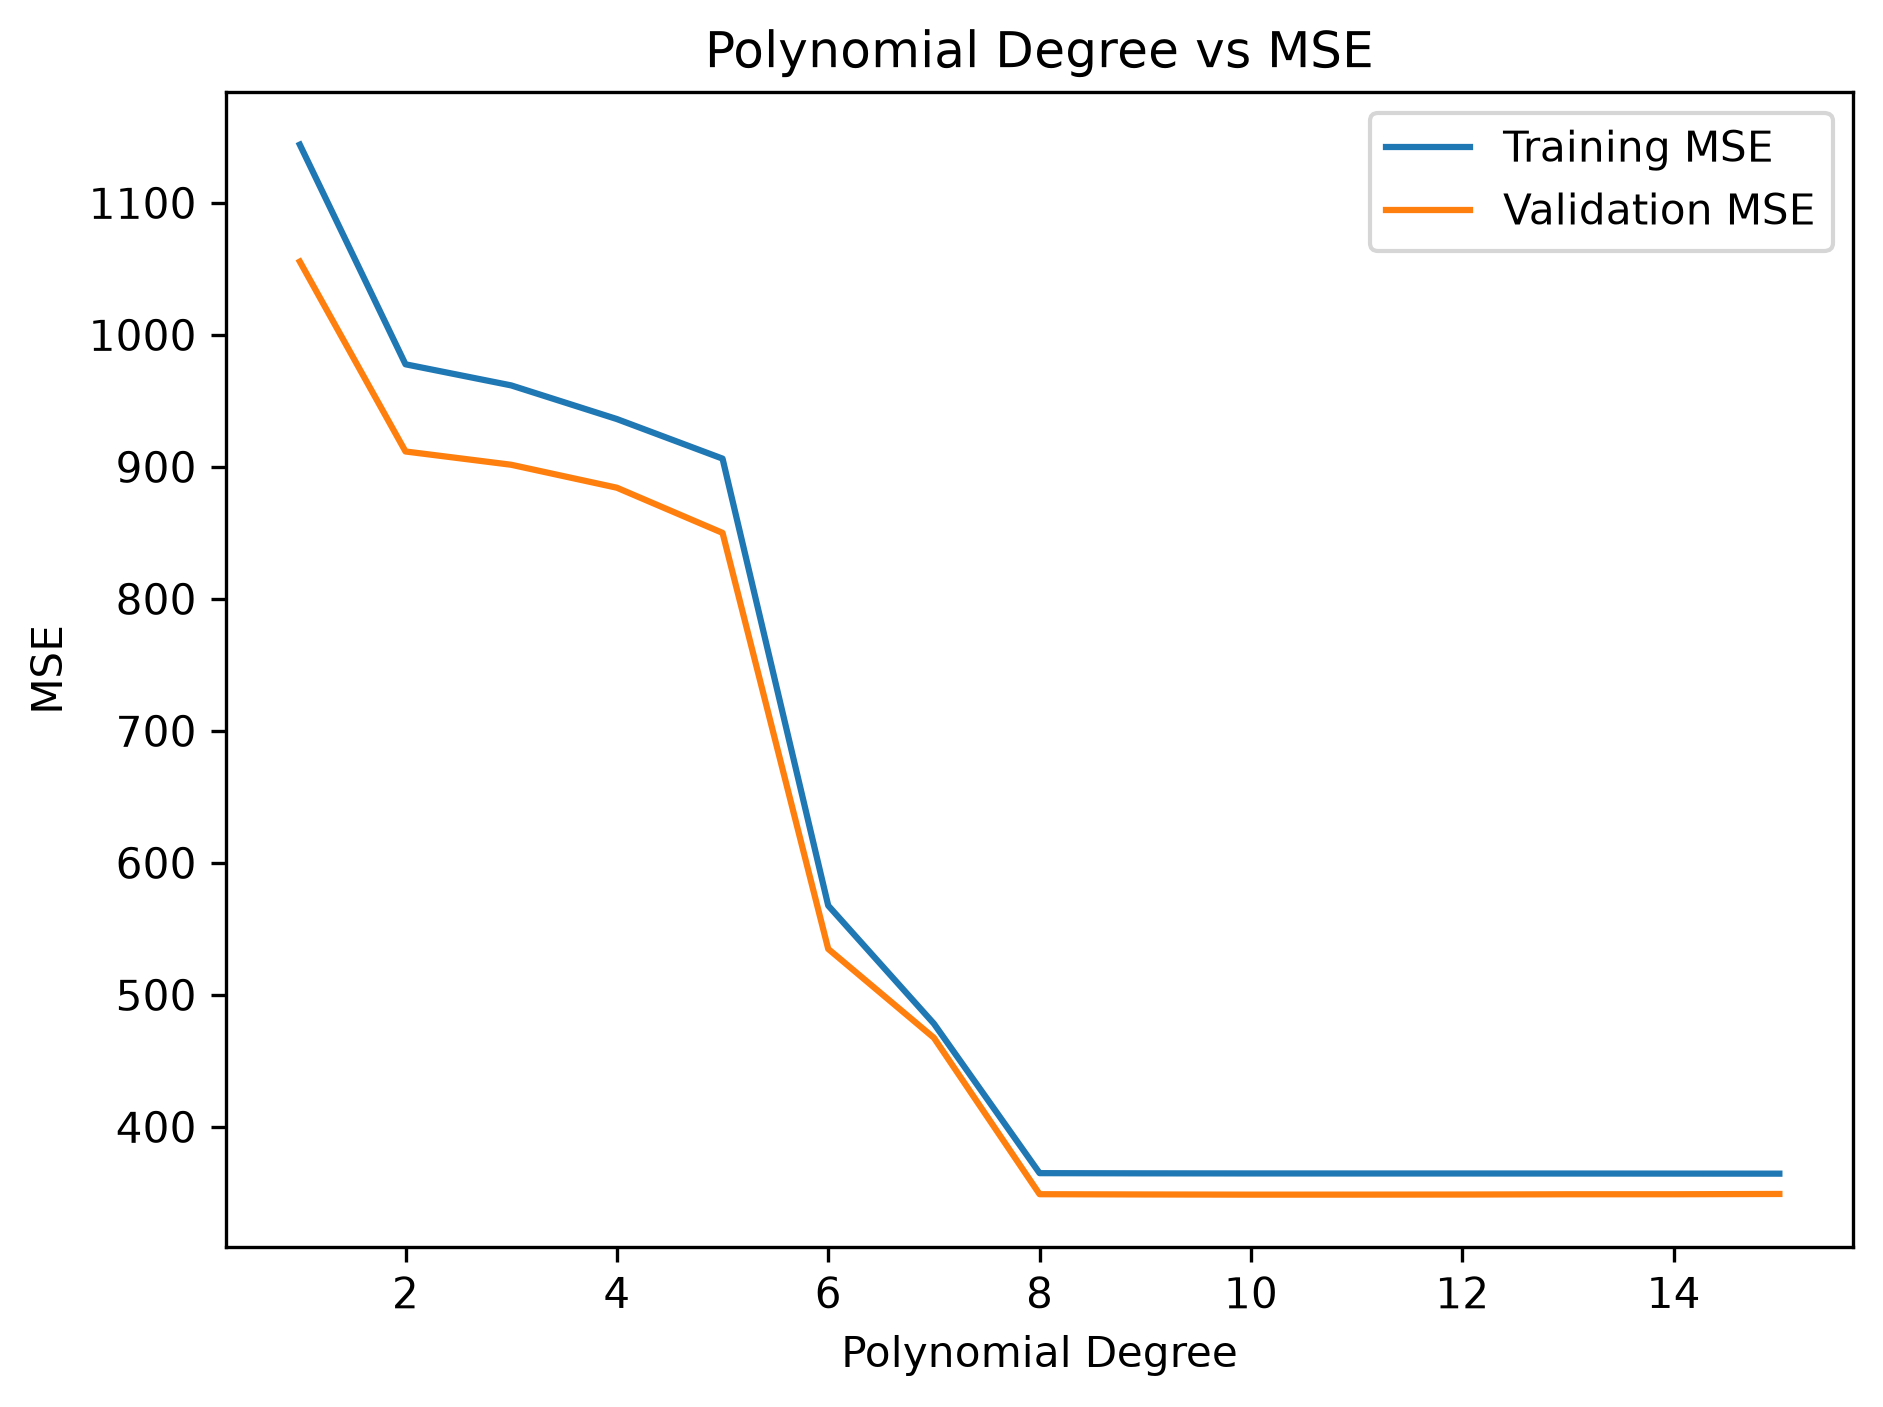
\includegraphics[width=0.82\textwidth]{degree_mse_comparison.png}
  \caption{Training and validation MSE for each polynomial degree.}
  \label{fig:degree-mse}
\end{figure}

\begin{table}[H]
  \centering
  \caption{Selected values from the degree comparison.}
  \begin{tabular}{rrr}
    \toprule
    Degree & Training MSE & Validation MSE \\
    \midrule
    1  & 1144.10 & 1055.51 \\
    5  & 906.23  & 849.98  \\
    8  & 364.92  & 348.96  \\
    10 & 364.69  & \textbf{348.63} \\
    15 & 364.53  & 349.14  \\
    \bottomrule
  \end{tabular}
\end{table}

We train the model on the train set and then we try out different degrees of polynomial basis on the validation set. Out of what we have tested above, Polynomial of degree 10 gave the lowest validation MSE. Thus, we choose degree 10 as the best polynomial degree.

\subsection*{Final evaluation}

The polynomial of degree 10 is modeled on the combined set of training and validation examples (8000 samples). That yields us Test MSE of $340.0071$.

\begin{figure}[H]
  \centering
  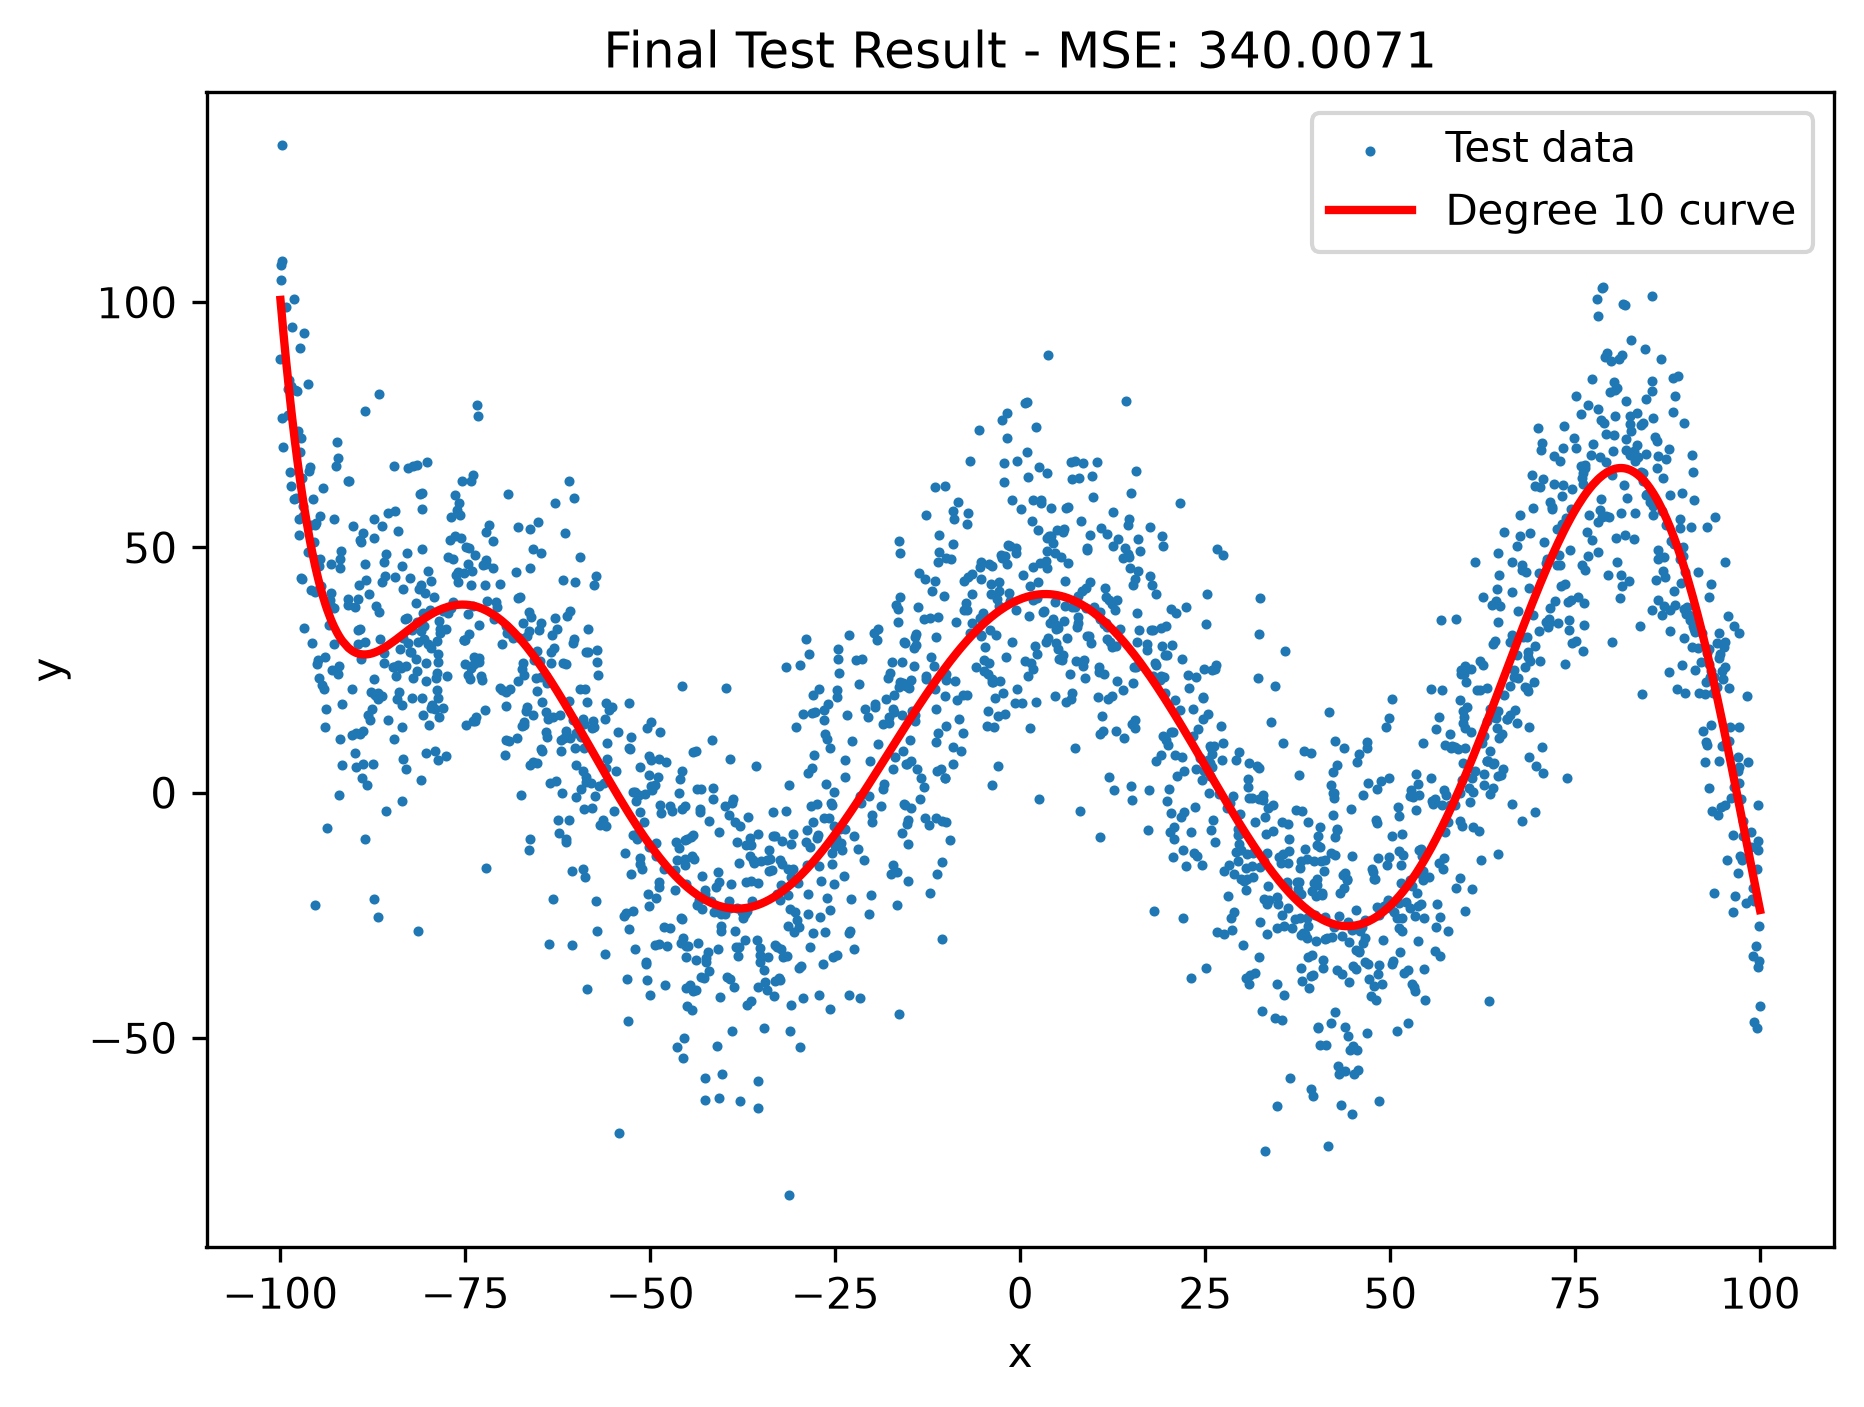
\includegraphics[width=0.82\textwidth]{test_fit_degree_10.png}
  \caption{Final degree-10 polynomial fit on the test set.}
  \label{fig:poly-test}
\end{figure}

\section*{ADDITIONAL EXPERIMENTS}

\subsection*{Polynomial basis without normalization}

The degree and the 80--20 final split were kept fixed. The unnormalized degree-10 model produced a test MSE of $340.0071$.

\begin{figure}[H]
  \centering
  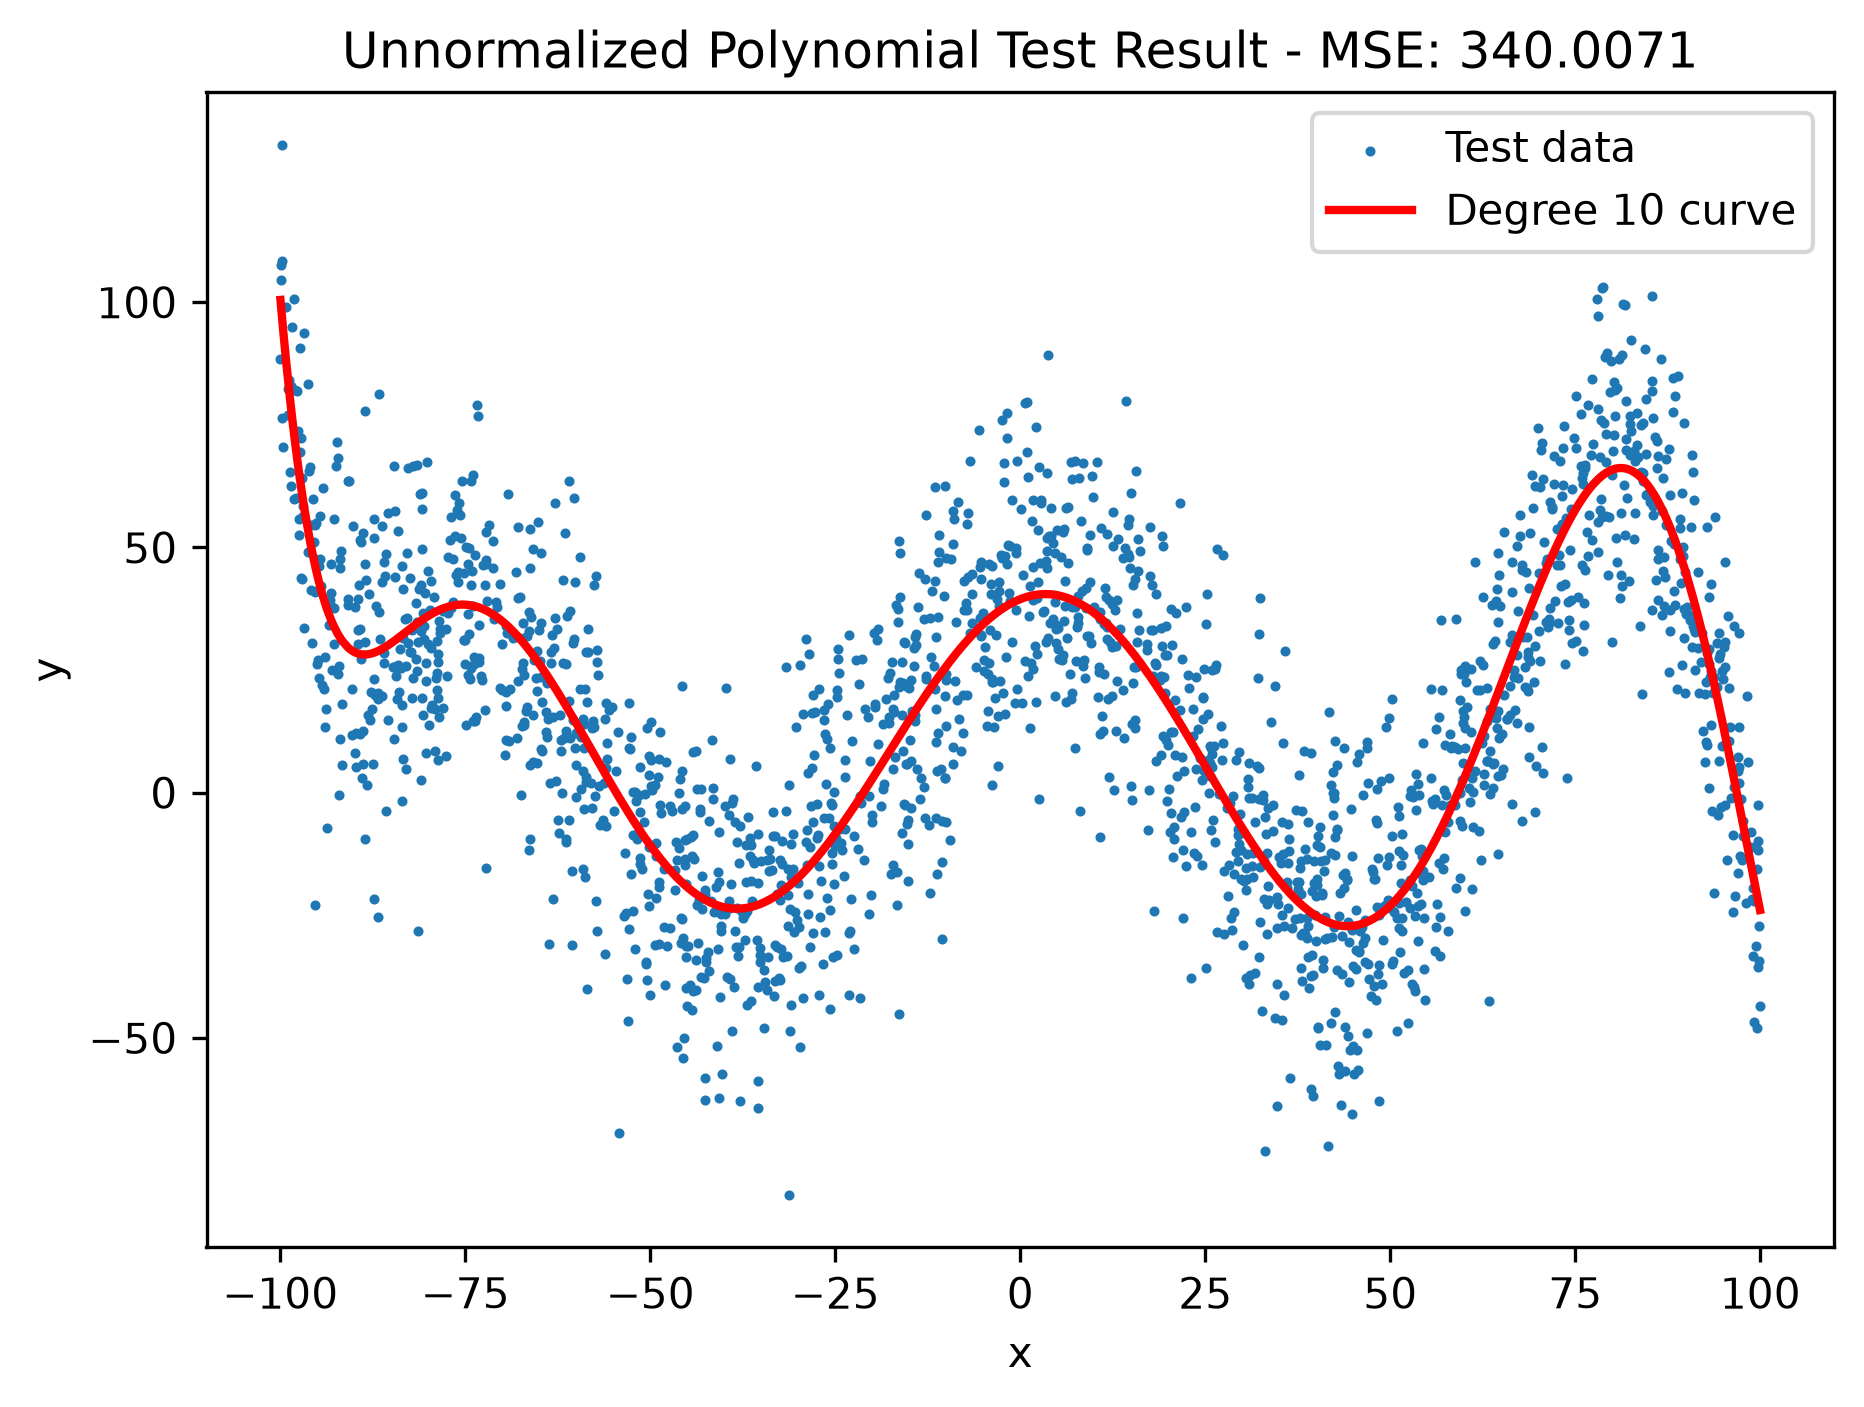
\includegraphics[width=0.82\textwidth]{unnormalized_polynomial_test_fit.png}
  \caption{Degree-10 polynomial fit without normalizing the input or target.}
  \label{fig:unnormalized-test}
\end{figure}

\begin{table}[H]
  \centering
  \caption{Examples of weights from the unnormalized polynomial model.}
  \begin{tabular}{lr}
    \toprule
    Weight & Value \\
    \midrule
    $w_0$  & $3.947\times10^{1}$ \\
    $w_5$  & $1.623\times10^{-7}$ \\
    $w_{10}$ & $2.457\times10^{-18}$ \\
    \bottomrule
  \end{tabular}
\end{table}

Both normalized and unnormalized version of polynomial regression yields us the same results. But, there is one particular thing that needs attention (i.e.) the weights. In the unnormalized version the weights had to get smaller in order to compensate for the large magnitude of input features as you can see $w_{10}$ is very small. But, the whole point of doing normalization is to improve the numerical stability while computation of least sqaures solutions. Because things like ${\boldsymbol{\Phi}^{\mathsf T}\boldsymbol{\Phi}}$ can easily have large values and that might cause problems like cutting of some floating point precision and etc... Usually it's a good thing to scale the values before you move on to modeling.

\subsection*{Gaussian basis}

For center $c_j$ and fixed width $\sigma$, the Gaussian basis function is

\begin{equation}
  \phi_j(x)=\exp\left\{-\frac{(x-c_j)^2}{2\sigma^2}\right\}.
  \label{eq:gaussian-basis}
\end{equation}

The design matrix is constructed with gaussian basis functions and equally spaced centers are chosen and we experiment with multiple center counts such as $5,10,15,20,25,30,$ and $35$.

\begin{figure}[H]
  \centering
  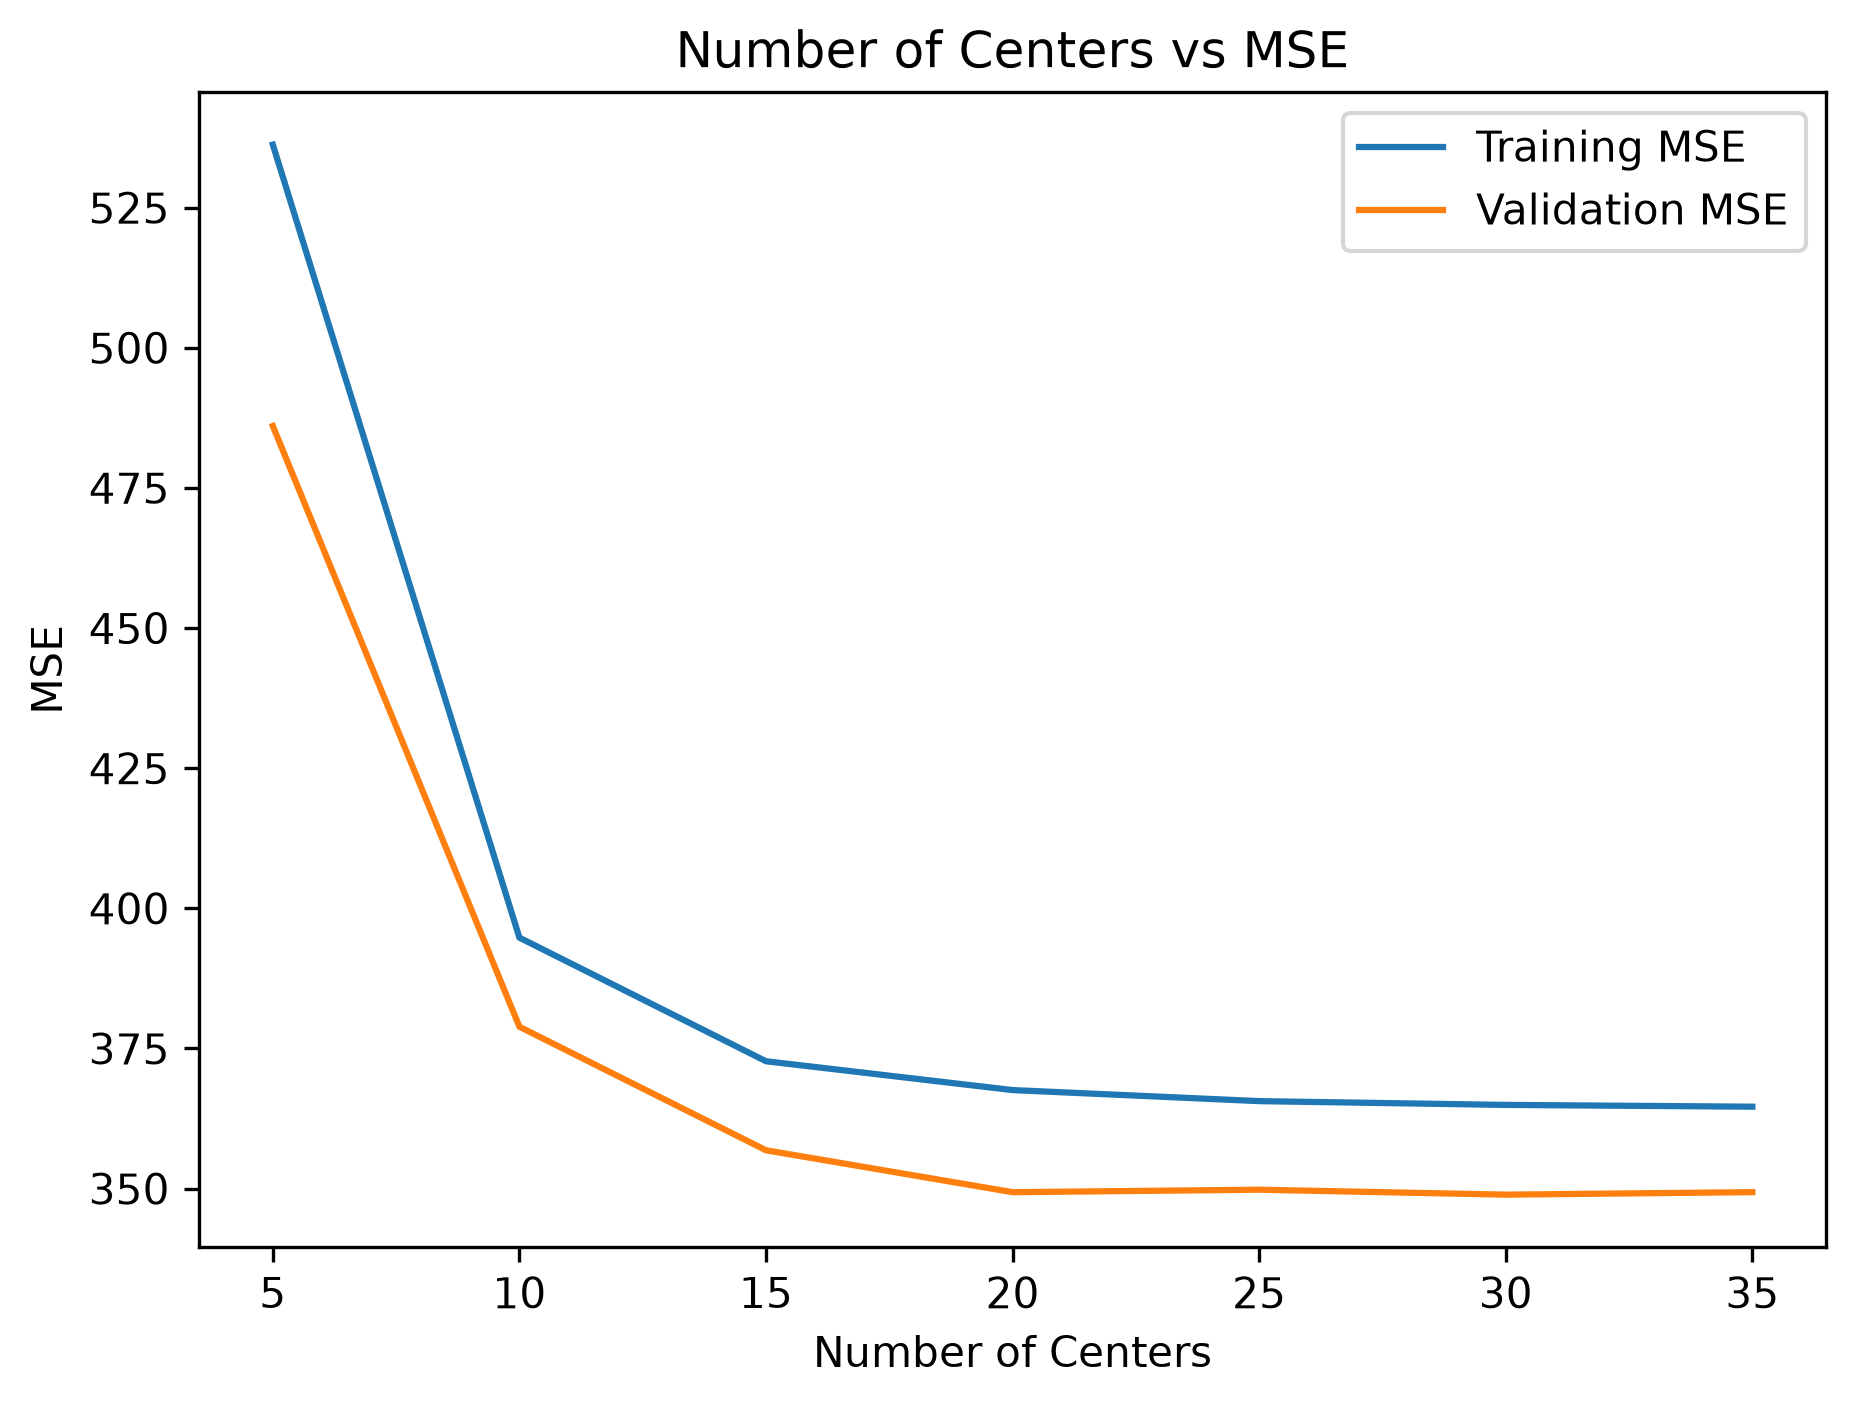
\includegraphics[width=0.82\textwidth]{gaussian_center_mse_comparison.png}
  \caption{Training and validation MSE for the candidate Gaussian centre counts.}
  \label{fig:gaussian-selection}
\end{figure}

The validation MSE becomes lowest when $348.9237$ at 30 centers. After combining the train and validation set we re-train the Gaussian model and obtain a test MSE of $342.1092$.

\begin{figure}[H]
  \centering
  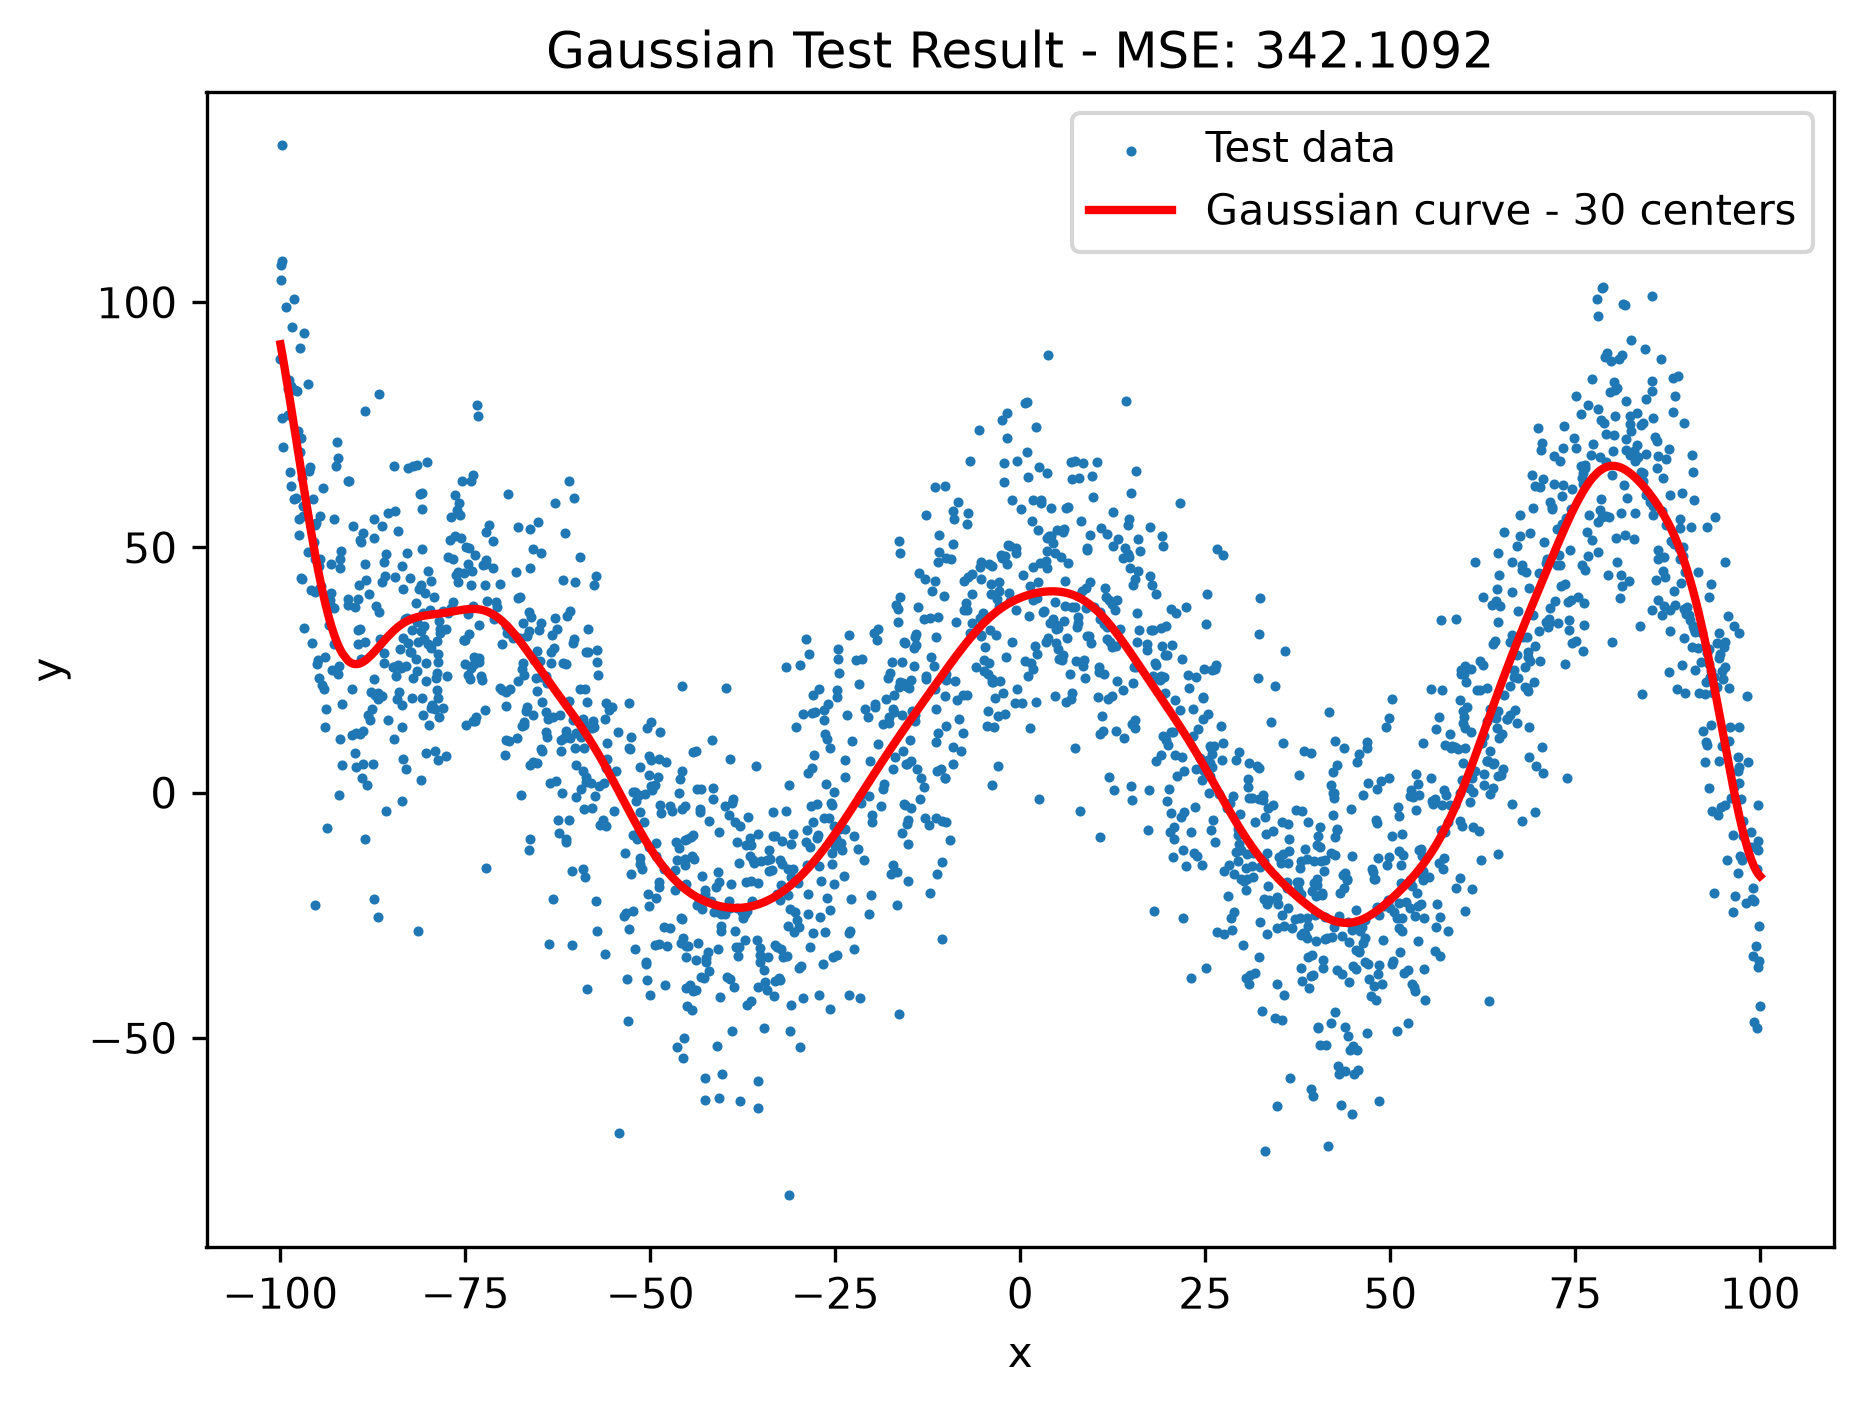
\includegraphics[width=0.82\textwidth]{gaussian_test_fit.png}
  \caption{Final 30-center Gaussian-basis fit on the test set.}
  \label{fig:gaussian-test}
\end{figure}

In gaussian basis it's all about centers and distances. If a point is away from the center it returns a low value and if a point in near the center it returns a high value. While the MSE came out to be pretty close to the polynomial basis, Visually the gaussian basis is very close to what polynomial basis have achieved. But from what we have tested, we could conclude among the 2 basis, Polynomial basis is performing better in this data.

\section*{INFERENCE}

\begin{table}[H]
  \centering
  \caption{Final comparison of the three fitted models.}
  \begin{tabular}{lrr}
    \toprule
    Model & Selected size & Test MSE \\
    \midrule
    Normalized polynomial & Degree 10 & 340.0071 \\
    Unnormalized polynomial & Degree 10 & 340.0071 \\
    Gaussian basis & 30 centers & 342.1092 \\
    \bottomrule
  \end{tabular}
\end{table}

The polynomial with the degree 10 learned the relationship better between the inputs and the outputs. Normalization doesn't particularly improve the the model. But, it changed the scale of the weights, which is expected as weights are just compensations that gets multiplied with inputs to reach the output. Gaussian basis with 30 centered performed considerably well. Polynomial basis performed slightly better while tested.

Overall this is experiment is a combination of learning new things and clearing out misconceptions. We learned how weights compensate for the inputs magnitude. Also, our misconceptions in the area of basis functions has been cleared. Like before we thought input feature matrix itself has multiple columns and they each get transformed via the basis function and get placed in their respective places. After this experiment, we came to know that a single feature vector in transformed into multiple features via basis function and that is a valuable learning experience.

\begin{thebibliography}{1}
\bibitem{bishop2006}
C. M. Bishop, \textit{Pattern Recognition and Machine Learning}, Springer, 2006, Chapter 3.
\end{thebibliography}

\end{document}
